\documentclass[sigconf]{acmart}
\settopmatter{printacmref=false} % Removes citation information below abstract
\renewcommand\footnotetextcopyrightpermission[1]{} % removes footnote with conference information in first column
\pagestyle{empty} % removes running headers
%%
%% \BibTeX command to typeset BibTeX logo in the docs
\AtBeginDocument{%
  \providecommand\BibTeX{{%
    \normalfont B\kern-0.5em{\scshape i\kern-0.25em b}\kern-0.8em\TeX}}}

\usepackage[linesnumbered,ruled]{algorithm2e}

\pagestyle{plain}
\graphicspath{ {../images/} }

\begin{document}


\title{Community Detection with ILS and GA-EDA}

\author{Aitor Zubillaga}
\affiliation{%
  \institution{UPV/EHU}
  \country{}}
\email{azubillaga012@ikasle.ehu.eus}

\author{Julen Etxaniz}
\affiliation{%
  \institution{UPV/EHU}
  \country{}}
\email{jetxaniz007@ikasle.ehu.eus}


%%
%% By default, the full list of authors will be used in the page
%% headers. Often, this list is too long, and will overlap
%% other information printed in the page headers. This command allows
%% the author to define a more concise list
%% of authors' names for this purpose.

%%
%% The abstract is a short summary of the work to be presented in the
%% article.
\begin{abstract}

Komunitateak detektatzea, orokorrean grafo egiturak erabiliz, azkeen urteetan indar handia hartzen ari den problema bat da. Hala eta guztiz ere ez da lortu behar bezalako soluzio bat. Artikulu honetan, bi algoritmo proposatzen dira grafoetan komunitateak detektatzeko: Iterated Local Search-en aldaera bat, eta Genetic Algorithm eta Estimation Distribution Algorithm-en arteko konbinazio bat. Emaitzen egokitasuna egiaztatzeko baseline bezala erabili den Random Search-ekin alderatuz, emaitza oso onak lortu dira.
\end{abstract}


\maketitle

\section{Sarrera eta motibazioa}

Azken urteetan sare sozialek indar handia hartu dute. Arrazoi nagusienetako bat, gure interesak partekatzen dituzten pertsonak aurkitzeko ematen dituzten erraztasunak dira \cite{clauset2004finding}. Interesak edo erlazioak partekatzen dituzten pertsonen multzoei komunitate deitzen zaie. Pertsona multzo batean komunitateak aurkitzeko gai izanez gero, posible da erabiltzaileari bere komunitate berdineko beste erabiltzaileei gogoko duten orrialdeen edo pertsonen gomendioak egitea, besteak beste. Hori dela eta, enpresak interes handia dute pertsonen artean komunitateak detektatzen.

Komunitateak islatzeko orokorrean grafo egiturak erabiltzen dira, non pertsona edo erabiltzaile bakoitza nodo bat den. Komunitateak elkarri oso loturik dauden nodoen bidez adieraziko genituzke. Lotura hauek nodo arteko ertzak dira. 
\ref{fig:graph}. irudian ikus daiteke adibide bat.

Gure probleman, NIPS kongresuan publikatzen duten autoreen komunitateak aztertu nahi ditugu. Zehazki, 2014 eta 2015 urteen bitartean, kongresu honetan eman diren elkarlan komunitate desberdinak aurkitu nahi ditugu. Komunitateak hainbat artikulu batera idatzi dituzten autoreek osatuko dituzte. Eta komunitate ezberdineko autoreen artean elkarlan gutxi egongo dira.

Lan honen helburua grafoetan komunitateak aurkitzeko bi algoritmo diseinatu eta aztertzea da. Bata soluzio bakarrean oinarritutakoa izango da, eta bestea poblazionala.

\begin{figure}
    \centering
    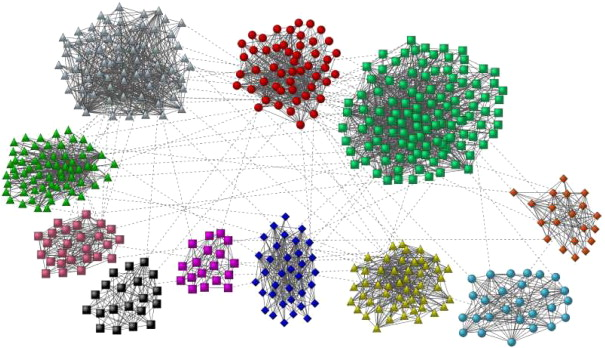
\includegraphics[width=0.7\linewidth]{example.jpg}
    \caption{Komunitateak grafo batean}
    \label{fig:graph}
\end{figure}


Bilaketa espazioa $\{1,...,k\}^n$ da, non $k$ komunitateak eta $n$ autoreak diren. Autore bakoitza zein komunitatekoa den zehaztuko dugu kodeketa horrekin. Beraz, autoreak komunitatetan banatzen dituen partizio onena aurkitzea izango da helburua. Onena zein den jakiteko, helburu-funtzio egoki bat definitu beharko dugu.

Lortutako emaitzak aztertzeko modularitatea erabiliko da \cite{clauset2004finding}. Modularitateak sare baten komunitate banaketaren egokitasuna neurtzen du. Banaketa egokia izango da komunitateen barruan ertz asko badaude, eta komunitate artean gutxi. Ausazko sare batean espero dezakegun modularitatea 0 da, eta modularitate maximoa 1 da. Beraz, gure helburua modularitatea maximizatzea izango da.

\begin{equation}
Q=\sum_{i} (e_{ii} - a_i^2).
\end{equation}

Lehenengo kantitateak $i$ komunitatetik hasita $j$ komunitatea lotzen duten ertzen pisuen frakzioa adierazten du:

\begin{equation}
e_{ij}=\frac{1}{2m}\sum_{vw}A_{vw}\delta(c_v,i)\delta(c_w,j).
\end{equation}

Bigarren kantitateak amaiera $i$ komunitateko nodoetan duten pisuen frakzioa adierazten du:

\begin{equation}
a_i=\frac{1}{2m}\sum_{v}k_v\delta(c_v,i).
\end{equation}

Aurreko bi ekuazioetako aldagaien esanahia honakoa da:
\begin{itemize}
    \item $A_{vw}$ $v$ nodotik $w$ nodora doan ertzaren pisua da.
    \item $c_v$ eta $c_w$ $v$ eta $w$ nodoen komunitatea dira.
    \item $\delta(i, j)$ 1 izango da $i = j$ bada eta 0 bestela.
    \item $m = \frac{1}{2}\sum_{vw}A_{vw}$ grafoko ertzen pixuen batura da.
    \item $k_v = \sum_{w}A_{vw}$ gradua erpin horri lotutako ertzen pixuen batura da.
\end{itemize}


\section{Algoritmoen diseinua}

Proiektu honetan bi algoritmo desberdin inplementatu dira, hauetako bat soluzio bakarrekoa eta bestea poblazionala.
Soluzio bakarreko algoritmoa ILS bat da. Algoritmo poblazionala aldiz GA-EDA algoritmoa inplementatu da. Bi algoritmoek hasierako soluzioak lortzeko metodo eraikitzaile estokastiko bat erabiltzen dute, Louvain algoritmoan oinarritzen dena. Beraz, hasteko Louvain azalduko da eta ondoren besteak.

\subsection{Louvain}
Louvain algoritmoaren \cite{blondel2008fast} pausuak \ref{fig:louvain}. irudian ikus daitezke. Iterazio bakoitzak bi fase ditu: batean komunitateen aldaketa lokala bakarrik eginda modularitatea optimizatzen saiatzen da eta bestean, aurkitutako komunitateak agregatzen dira komunitateen sare berri bat sortzeko. Iterazio hauek modularitatea hobetzea posible ez den arte errepikatzen dira.

Community moduluko \texttt{generate\_dendogram} funtzioak, komunitateak elkartzen ditu, hauek elkartzearen ondorioz modularitatea hobetzen bada bakarrik. Beraz, komunitate kopuru optimora iritsitakoan gelditu egiten da. Gure kasuan aldiz, emandako komunitate kopurura iristea interesatzen zaigu, nahiz eta beste komunitate kopuru batekin modularitate hobea lortzea posible izan. Hori dela eta aldaketak egin dira \texttt{best\_partition} funtzioan, alde batetik, deseatutako komunitate kopurura iritsitakoan algoritmoa gelditzeko, eta beste aldetik, nahiz eta soluzio optimoa aurkitu, modularitatea ahal den gutxiena txartuz, desiratzen den komunitate kopurura iritsi ahal izateko.

Hala eta guztiz ere, ezin da lortu proiektu honetan erabili den instantziarekin komunitate kopurua $279$tik jaistea, izan ere, komunitateen artean ertz gehiago ez baitago.

Hori konpontzeko, \texttt{best\_fixed\_partition} funtzioa inplementatu dugu. Honek, lehenengo \texttt{best\_partition} funtzioari deituko dio. Honek, jasotzen duen soluzioari, soberan dituen komunitate txikienak hartu eta guztiak komunitate berean elkartuko dizkio. Izan ere, komunitateen artean konexiorik ez dagoenean, ahal den modularitate hoberena lortzeko modurik onena komunitate txikienak elkartzea da, komunitate handiak eragin handiago baitute modularitatean eta hauek txartzeak beraz, asko jaisten baitu fitnessa. Komunitate txikienak non elkartu aukeratzeko, aukera guztiak aztertu eta onena aukeratzen da.

\begin{figure}
    \centering
    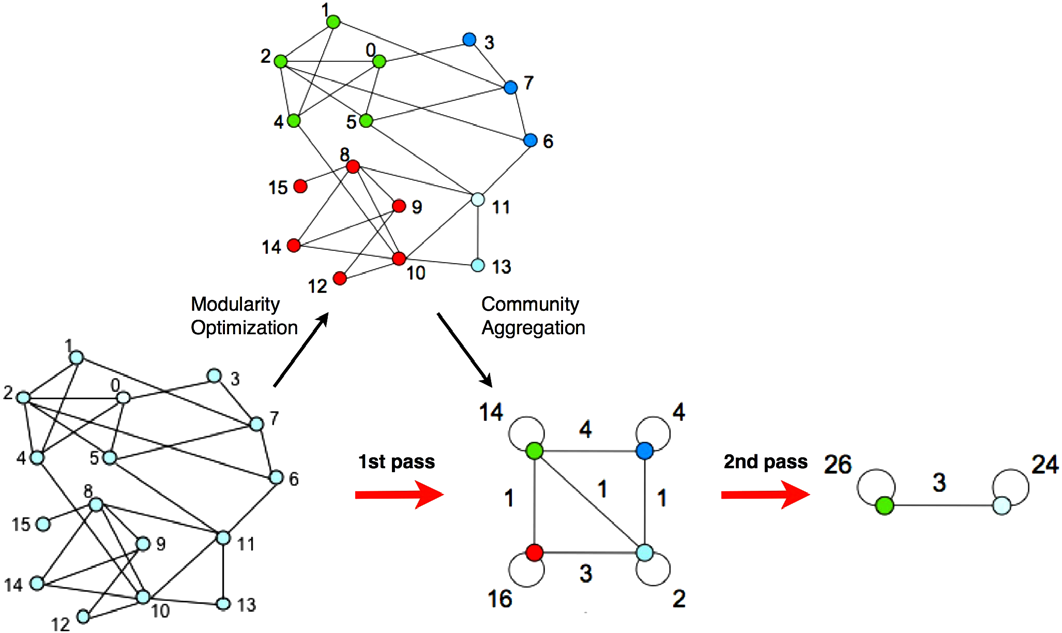
\includegraphics[width=\linewidth]{Louvain}
    \caption{Louvain algoritmoa: Iterazio bakoitzak bi fase ditu, aldaketa lokala eta komunitateen agregazioa.}
    \label{fig:louvain}
\end{figure}

\subsection{ILS}
Iterated Local Search \cite{liu2020iterated} soluzio bakarreko algoritmoa inplementatu da. Hasierako soluzioa sortzeko Louvain eraikitzailea erabiltzen da. Ondoren, perturbazioak sartu, bilaketa lokala egiten da eta soluzioa eguneratzen da. \ref{alg:ils}. algoritmoan ikus daiteke pseudokodea.

\begin{algorithm}
    \SetKwInOut{Input}{Input}
    \SetKwInOut{Output}{Output}
    \Input{$local\_search$ bilaketa algoritmoa, $perturbation$ perturbazioa, $simmulated\_annealing$ onarpen-baldintza eta $stop\_criterion$ gelditzeko irizpidea}
    \Output{$s^*$ soluzioa}
    \While{$!stop\_criterion()$}{
        $s^* = perturbation(s^*)$
        
        $s = local\_search(s^*)$
        
        $s^* = simmulated\_annealing(s)$
    }
    \caption{ILS}
    \label{alg:ils}
\end{algorithm}

Perturbatzeko, lehenik soluzioan 2 komunitate ausaz hartu eta elkartu egiten dira, eta ondoren komunitate bat ausaz hartu eta ausaz aukeratutako bi zatitan banatzen da. Funtzioak jasotako graduak, soluzioa zenbat aldiz perturbatuko den zehazten du. 

Behin perturbazioa sortuta, soluzio honen optimo lokala aurkituko da best first estrategia eta Swap ingurune funtzioa erabiliz. Emaitza eguneratzeko Simulated Annealing estrategia erabiltzen du, emaitza txarragoak onartu ahal izateko. Gero eta tenperatura handiagoa, orduan eta probabilitate hanfiagoa dago emaitza txarrak onartzeko. Hasierako tenperatura eta tenperatura egokitzeko modua, \ref{espe} azpiatalean azalduko da.

\subsection{GA-EDA}
GA-EDA \cite{pena2004ga} populaziotan oinarritutako algoritmoa inplementatu da. Algoritmo honek Genetic Algorithms eta Estimation of Distribution Algorithms konbinatzen ditu. Bi algoritmo hauek antzekotasun asko dituzte, baina biak konbinatzean populazioetan dibertsitate gehiago eta emaitza hobeak lor daitezke. \ref{alg:ga_eda}. pseudokodean eta \ref{fig:ga_eda}. irudian ikus daitezke honen funtzionamedua.

\begin{figure}
    \centering
    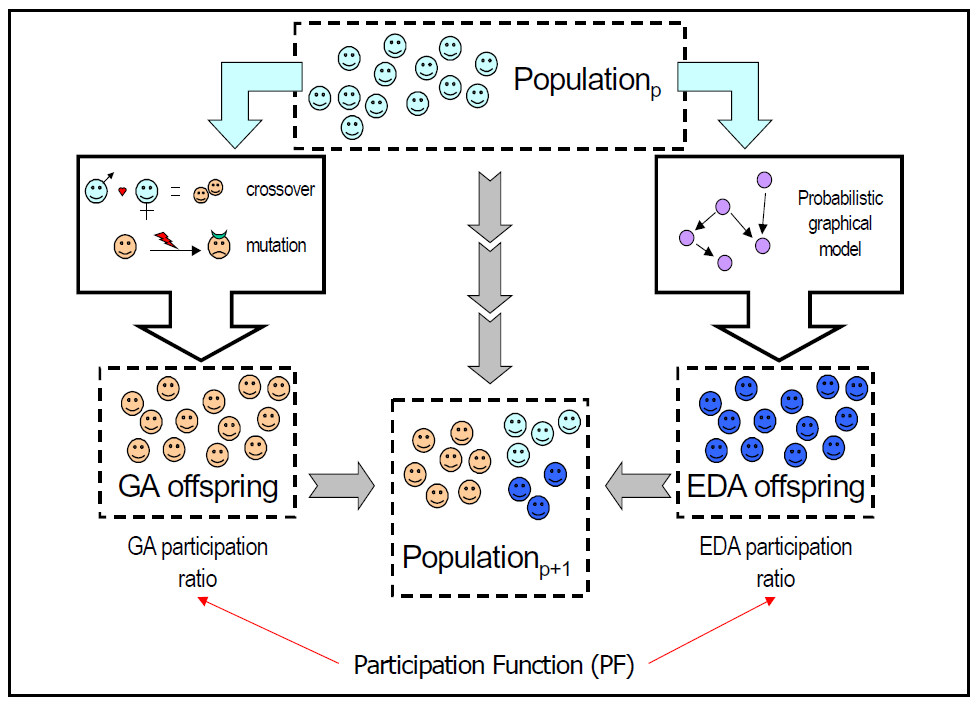
\includegraphics[width=\linewidth]{GA-EDA}
    \caption{GA-EDA algoritmoan iterazio bat nola osatzen den ikus daiteke.}
    \label{fig:ga_eda}
\end{figure}

Hasteko, hasierako populazioa eraikitzen da, ausaz edo moldatutako Louvain heuristikoa erabiliz. Gero, hainbat iterazio egiten dira, ebaluazio kopuru maximora iritsi arte. Iterazio bakoitzean pauso berdinak errepikatuko dira. Amaitzeko, populazioko soluzio onena itzultzen da.  

\begin{itemize}
    \item Selection eragiketan hainbat soluzio aukeratzen dira aurreko populaziotik. \texttt{best\_selection} aukeraketan beti soluzio onenak aukeratzen dira.  \texttt{roulette\_selection} aukeraketan soluzioen probabilitateak kalkulatzeko fitness balioa erabiltzen da.
    
    \texttt{rank\_selection} aukeraketan soluzioen probabilitateak kalkulatzeko ranking-eko posizioa erabiltzen da. \texttt{tournament\_selection} aukeraketan hainbat txapelketa egiten dira soluzioak ausaz aukeratuz.
    \item Crossover eragiketan aukeratutako soluzioak birkonbinatzen dira soluzio berriak sortzeko. \texttt{one\_point\_crossover} algoritmoan soluzioko puntu bat aukeratzen da. Puntu horretatik eskuinera dagoen soluzio zatia trukatzen da bi soluzioetan soluzio berriak sortuz.
    \item Mutation eragiketan, aurreko soluzioei mutazio bat egiten zaie probabilitate batekin. \texttt{bit\_mutation} eragiketan soluzioen posizio bakoitzaren balioa ausaz aldatzen da.
    \item Learning eragiketan, aukeratutako soluzioak erabilita eredu probabilistikoaren parametroak ikasten dira.
    \item Sampling eragiketan, ikasitako eredutik abiatuta soluzio berriak lagindu eta ebaluatzen dira.
    \item Update eragiketan, soluzio berrien eta aurrekoen artetik soluzio batzuk gordetzen dira. \texttt{elistism\_update} eragiketak aurreko populazioko soluzio onena gordetzen du eta populazio berriko onenak. \texttt{elistism\_update} eragiketak aurreko populazioko eta populazio berriko soluzioak elkartzen ditu eta onenak aukeratzen ditu.
\end{itemize}

\begin{algorithm}
    \SetKwInOut{Input}{Input}
    \SetKwInOut{Output}{Output}
    \Input{$evaluate$, $select$, $learn$, $reproduce$, $sample$, $update$ eta $stop\_criterion$ operadoreak, $P_0$ hasierako populazioa}
    \Output{$s^*$ soluzioa}
    \While{$!stop\_criterion()$}{
        $f_t = evaluate(P_t)$
        
        $P^s_t = select(P_t, f_t)$
        
        $P^g_t = reproduce(P^s_t)$
        
        $P^e_t = sample(M_t)$
        
        $P_{t+1} = update(P_t, P^g_t, P^e_t)$
        
        $t = t + 1$
    }
    $s^* =$ Populazioko soluziorik onena
    \caption{GA-EDA}
    \label{alg:ga_eda}
\end{algorithm}

\section{Esperimentazioa}

Esperimentazioak bi fase izango ditu. Lehenengo fasean, ILS eta GA-EDA algoritmoen parametroak kalibratuko ditugu. Bigarren fasean, algoritmoak konparatuko ditugu 2 komunitatetik 100 komunitatera arte. Beti ere, jakiteko gure algoritmoak onak edo txarrak diren, RS baseline algoritmoa erabiliko dugu.

\subsection{Parametroak kalibratu}
\label{espe}
Parametroak kalibratzeko Grid Search erabili dugu. Parametro garrantzitsuenetan hainbat balio posible definitu ditu eta beraien arteko konbinaketa denak probatu. Komunitate kopuruari dagokionez, muturreko kasuak bakarrik probatu ditugu, 2 eta 100 komunitate. 50 komunitaterekin ere probatu dugu baina antzekoak zirenez denbora aurrezteko kendu dugu. Gainerako parametroak gure ustez egokia den balio estatiko batean utzi ditugu. Izan ere, exekuzioak egiteko denbora asko behar da, eta luzea da parametro guztiak kalibratzea. 

Parametro aukera bakoitzerako $10^4$ ebaluazio eta 5 errepikapen egin ditugu. Errepikapen bakoitzeko fitness eta denbora balioaekin batazbestekoak kalkulatu ditugu. Fitness-en batazbesteko balioekin heatmap motako grafikak atera ditugu. 

ILS algoritmoan komunitate kopuru bakoitzerako 6 parametro konbinazio probatu ditugu. Zehazki, perturbazio gradurako $\{1, 3, 5\}$ balioak eta simmulated annealing-en hasierako tenperaturarako $\{0.0001, 0.001\}$. Tenperatura eguneratzeko $0.9$ balioarekin bidertzen dugu beti. Bi komunitate kopuruetarako emaitza onena $3$ eta $0.001$ parametroekin lortu ditugu. \ref{fig:heatmap}. irudian ikus daitezke 2 komunitaterako balioak.Beraz, esperimentazioaren hurrengo faserako parametro horiek erabiliko ditugu. 

\begin{figure}
    \centering
    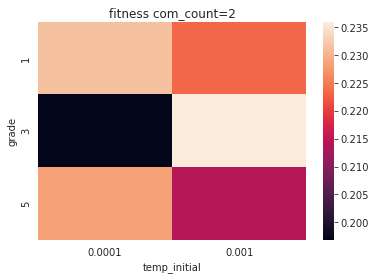
\includegraphics[width=0.6\linewidth]{heatmap}
    \caption{ILS algoritmoaren parametroen heatmapa 2 komunitaterekin.}
    \label{fig:heatmap}
\end{figure}

GA-EDA algoritmoan, berriz, 4 parametro konbinazio probatu ditugu. Populazio tamainarako $\{30, 40\}$ eta aukeraketa tamainarako $\{15, 20\}$. Komunitate kopurua 2 denean, $30$ eta $15$ balioekin lortzen da fitness altuena. 100 komunitaterekin onena ez den arren, denak antzekoak dira. Gainera, denbora aldetik azkarrena da, soluzio kopurua txikiagoa delako. Ondorioz, parametro horiek erabiliko ditugu konparaketan.

Gainerako parametroei dagokionez, balio estatikoak aukeratu ditugu. Offspring tamainak populazio tamainaren erdira finkatu ditugu, hau da, $15$. Mutazio probabilitatea $0.01$-en ezarri dugu. Hasierako populazioa sortzeko \texttt{louvain\_population}, aukeraketarako \texttt{roulette\_selection}, eguneratzeko \texttt{elitism\_selection}, birkonbinaziorako \texttt{one\_point\_crossover} eta mutaziorako \texttt{bit\_mutation}.

\subsection{Algoritmoak konparatu}
Hiru algoritmoen konparaketa egiteko, komunitate kopuru bakoitzerako $10^4$ ebaluazio eta 5 errepikapen egin ditugu. Guztira 11 komunitate kopuru desberdin probatu ditugu, $2, 10, 20, ..., 100$. Fitness eta denbora emaitzekin boxplot motako grafikak atera ditugu, x ardatzean komunitate kopurua jarriz. Gainera, fitness emaitzen batazbestekoak \ref{tab:results}. taulan ikus daitezke.

\begin{table}[ht]
\centering
\begin{tabular}{|c|c|c|c|} 
    \hline
    Komunitateak & RS & ILS & GA-EDA \\
    \hline
    2 & 0.0021 & 0.1924 & 0.3131 \\
    10 & -0.0038 & 0.7184 & 0.7344 \\
    20 & 0.0001 & 0.8082 & 0.8128 \\
    30 & -0.0018 & 0.8552 & 0.8593 \\
    40 & 0.0008 & 0.8841 & 0.8866 \\
    50 & 0.0009 & 0.9000 & 0.9087 \\
    60 & -0.0001 & 0.9154 & 0.9238 \\
    70 & 0.0001 & 0.9249 & 0.9342 \\
    80 & 0.0003 & 0.9348 & 0.9406 \\
    90 & -0.0009 & 0.9389 & 0.9451 \\
    100 & -0.0002 & 0.9387 & 0.9495 \\
    \hline
\end{tabular}
\caption{Batazbesteko fitness balioak 3 algoritmoetan komunitate kopuru bakoitzerako.}
\label{tab:results}
\end{table}

Fitness-ari dagokionez, ILS eta GA-EDA askoz hobeak direla ikus daiteke. Eta horien artean GA-EDA pixkat hobea da komunitate kopuru guztietarako. Orokorrean, bariantza txikia da eta horregatik kutxa batzuk ia ez dira ikusten. Ikusi \ref{fig:boxplot_fitness}. irudia.

\begin{figure}
    \centering
    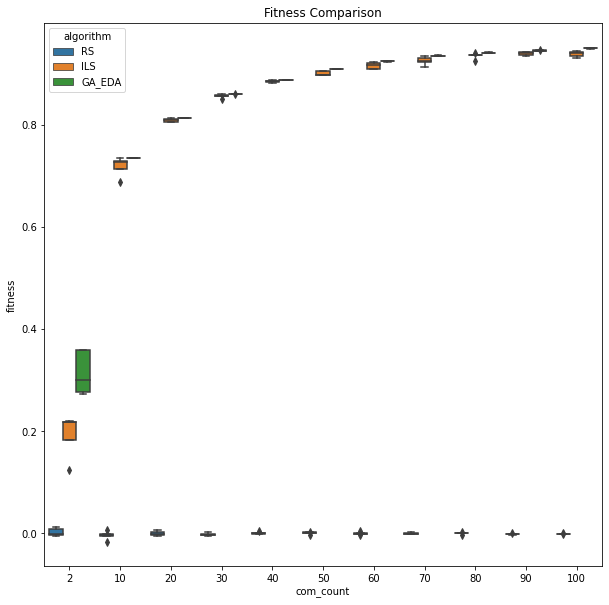
\includegraphics[width=1\linewidth]{boxplot_fitness}
    \caption{Fitness-aren boxplota 3 algoritmoekin komunitate kopuru bakoitzerako.}
    \label{fig:boxplot_fitness}
\end{figure}

Analisi estatistiko Bayesiarra ere gauzatu dugu ILS eta GA-EDA algoritmoak konparatzeko. Honetarako, bi algoritmoen artean berdinketa dagoela erabaki dugu aldea $5*10^{-3}$ baino txikiagoa denean. Analisiaren emaitzak \ref{fig:boxplot_fitness}. irudian ikus daitezke. Laburbilduz, GA-EDA hobea izateko probabilitatea 0.698 da, berdinak izatekoa 0.301 eta okerragoa izatekoa 0.000.

\begin{figure}
    \centering
    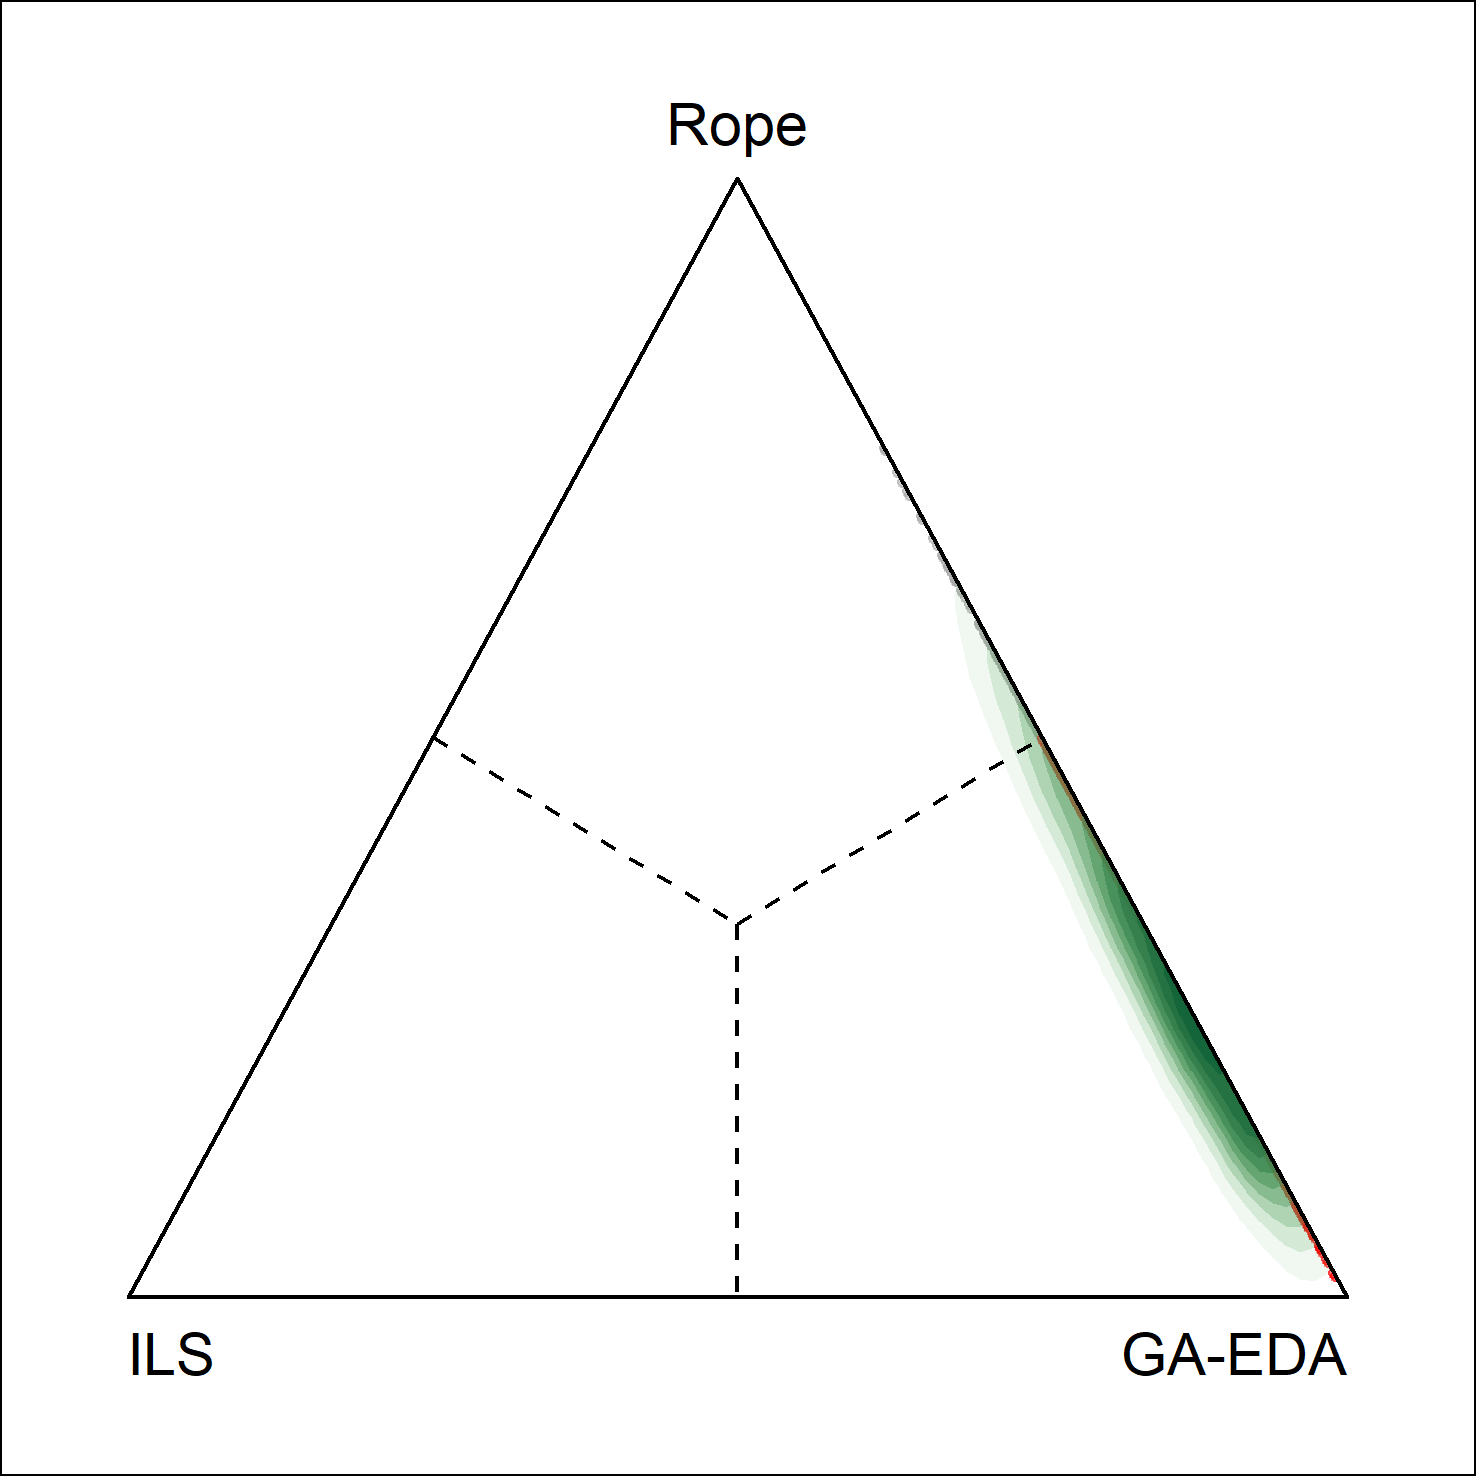
\includegraphics[width=0.5\linewidth]{simplex}
    \caption{Simplex grafikoa ILS eta GA-EDA algoritmoen irabazteko, berdintzeko eta berdintzeko probabilitateekin.}
    \label{fig:simplex}
\end{figure}

Denborari dagokionez, ILS eta RS askoz azkarragoak dira GA-EDArekin konparatuz. Komunitate kopurua handitu ahala, GA-EDAk behar duen denbora handitzen joaten da. Beste bi algoritmoetan, berriz, gutxi gorabehera mantendu egiten da. Ikusi \ref{fig:boxplot_time}. irudia.

\begin{figure}
    \centering
    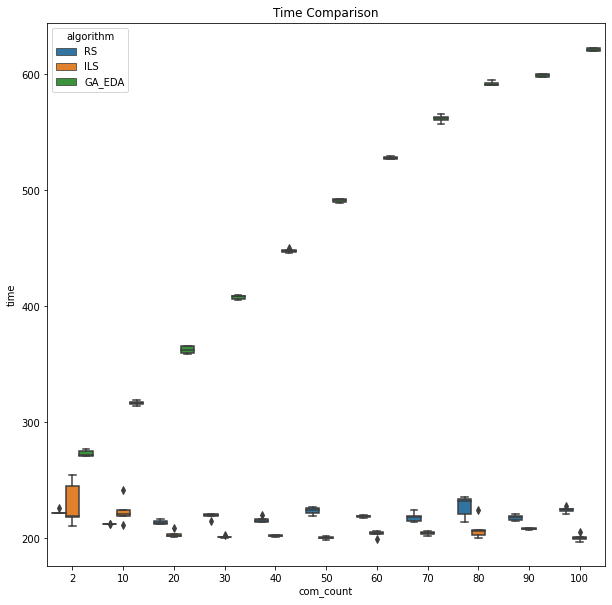
\includegraphics[width=1\linewidth]{boxplot_time}
    \caption{Denboraren boxplota 3 algoritmoekin komunitate kopuru bakoitzerako.}
    \label{fig:boxplot_time}
\end{figure}

\section{Ondorioak}
Azken urteetan komunitateak detektatzeak indar handia hartu du, batik bat sare sozialen hazkundea dela eta. Artikulu honetan, bi algoritmo proposatu dira grafoetan komunitateak detektatzeko: bata ILS-ren aldaera, eta bestea GA-EDA. Emaitzen egokitasuna egiaztatzeko, Random Search erabili da baseline bezala. Honekin alderatuz emaitza onak lortu dira bi algoritmoekin. Alde batetik, GA-EDAk emaitza apur bat hobeak lortzen ditu, batik bat komunitate kopurua oso mugatua denean. Bestalde, ILS algoritmoa eraginkorragoa da denbora askoz gutxiago behar baitu soluzio egokietara iristeko.

Lan honen mugak kontuan hartuz etorkizunean hainbat hobekuntza egin daitezke. Algoritmoen parametroak kalibratzerakoan aukera gutxi probatu dira denbora murriztapenen ondorioz. Proba gehiago egiteko exekuzio denbora gehiago murriztea komeniko litzateke. Honetaz gain, $10^4$ ebaluazio egin ordez $10^5$ edo $10^6$ ebaluazio egitea hobe izango litzateke. Era berean, errepikapen kopurua ere gutxienez $10$era handitzea komenigarria izango litzateke.

\bibliographystyle{ACM-Reference-Format}
\bibliography{community}

\end{document}
\endinput
